\documentclass{article}
\usepackage{ctex}
\usepackage{enumerate}
\usepackage{enumitem}
\usepackage{graphicx}
\usepackage{color}
\usepackage{hyperref}
\usepackage{textcomp}
\usepackage[T1]{fontenc}
\usepackage[utf8]{inputenc}
\usepackage[english]{babel}
\usepackage[svgnames]{xcolor}
\usepackage{listings}
\usepackage{lmodern}
\setlist[enumerate,1]{label=(\arabic*).,font=\textup,
leftmargin=7mm,labelsep=1.5mm,topsep=0mm,itemsep=-0.8mm}
%%%%%%%%%%%%%%%%%%%%%%%%%%%%%%%%%%%%%%%%%
% Lachaise Assignment
% Structure Specification File
% Version 1.0 (26/6/2018)
%
% This template originates from:
% http://www.LaTeXTemplates.com
%
% Authors:
% Marion Lachaise & François Févotte
% Vel (vel@LaTeXTemplates.com)
%
% License:
% CC BY-NC-SA 3.0 (http://creativecommons.org/licenses/by-nc-sa/3.0/)
% 
%%%%%%%%%%%%%%%%%%%%%%%%%%%%%%%%%%%%%%%%%

%----------------------------------------------------------------------------------------
%	PACKAGES AND OTHER DOCUMENT CONFIGURATIONS
%----------------------------------------------------------------------------------------

\usepackage{amsmath,amsfonts,stmaryrd,amssymb} % Math packages

\usepackage{enumerate} % Custom item numbers for enumerations

\usepackage[ruled]{algorithm2e} % Algorithms

\usepackage[framemethod=tikz]{mdframed} % Allows defining custom boxed/framed environments

\usepackage{listings} % File listings, with syntax highlighting
\lstset{
	basicstyle=\ttfamily, % Typeset listings in monospace font
}

%----------------------------------------------------------------------------------------
%	DOCUMENT MARGINS
%----------------------------------------------------------------------------------------

\usepackage{geometry} % Required for adjusting page dimensions and margins

\geometry{
	paper=a4paper, % Paper size, change to letterpaper for US letter size
	top=2.5cm, % Top margin
	bottom=3cm, % Bottom margin
	left=2.5cm, % Left margin
	right=2.5cm, % Right margin
	headheight=14pt, % Header height
	footskip=1.5cm, % Space from the bottom margin to the baseline of the footer
	headsep=1.2cm, % Space from the top margin to the baseline of the header
	%showframe, % Uncomment to show how the type block is set on the page
}

%----------------------------------------------------------------------------------------
%	FONTS
%----------------------------------------------------------------------------------------

\usepackage[utf8]{inputenc} % Required for inputting international characters
\usepackage[T1]{fontenc} % Output font encoding for international characters

\usepackage{XCharter} % Use the XCharter fonts

%----------------------------------------------------------------------------------------
%	COMMAND LINE ENVIRONMENT
%----------------------------------------------------------------------------------------

% Usage:
% \begin{commandline}
%	\begin{verbatim}
%		$ ls
%		
%		Applications	Desktop	...
%	\end{verbatim}
% \end{commandline}

\mdfdefinestyle{commandline}{
	leftmargin=10pt,
	rightmargin=10pt,
	innerleftmargin=15pt,
	middlelinecolor=black!50!white,
	middlelinewidth=2pt,
	frametitlerule=false,
	backgroundcolor=black!5!white,
	frametitle={Command Line},
	frametitlefont={\normalfont\sffamily\color{white}\hspace{-1em}},
	frametitlebackgroundcolor=black!50!white,
	nobreak,
}

% Define a custom environment for command-line snapshots
\newenvironment{commandline}{
	\medskip
	\begin{mdframed}[style=commandline]
}{
	\end{mdframed}
	\medskip
}

%----------------------------------------------------------------------------------------
%	FILE CONTENTS ENVIRONMENT
%----------------------------------------------------------------------------------------

% Usage:
% \begin{file}[optional filename, defaults to "File"]
%	File contents, for example, with a listings environment
% \end{file}

\mdfdefinestyle{file}{
	innertopmargin=1.6\baselineskip,
	innerbottommargin=0.8\baselineskip,
	topline=false, bottomline=false,
	leftline=false, rightline=false,
	leftmargin=2cm,
	rightmargin=2cm,
	singleextra={%
		\draw[fill=black!10!white](P)++(0,-1.2em)rectangle(P-|O);
		\node[anchor=north west]
		at(P-|O){\ttfamily\mdfilename};
		%
		\def\l{3em}
		\draw(O-|P)++(-\l,0)--++(\l,\l)--(P)--(P-|O)--(O)--cycle;
		\draw(O-|P)++(-\l,0)--++(0,\l)--++(\l,0);
	},
	nobreak,
}

% Define a custom environment for file contents
\newenvironment{file}[1][File]{ % Set the default filename to "File"
	\medskip
	\newcommand{\mdfilename}{#1}
	\begin{mdframed}[style=file]
}{
	\end{mdframed}
	\medskip
}

%----------------------------------------------------------------------------------------
%	NUMBERED QUESTIONS ENVIRONMENT
%----------------------------------------------------------------------------------------

% Usage:
% \begin{question}[optional title]
%	Question contents
% \end{question}

\mdfdefinestyle{question}{
	innertopmargin=1.2\baselineskip,
	innerbottommargin=0.8\baselineskip,
	roundcorner=5pt,
	nobreak,
	singleextra={%
		\draw(P-|O)node[xshift=1em,anchor=west,fill=white,draw,rounded corners=5pt]{%
		Question \theQuestion\questionTitle};
	},
}

\newcounter{Question} % Stores the current question number that gets iterated with each new question

% Define a custom environment for numbered questions
\newenvironment{question}[1][\unskip]{
	\bigskip
	\stepcounter{Question}
	\newcommand{\questionTitle}{~#1}
	\begin{mdframed}[style=question]
}{
	\end{mdframed}
	\medskip
}

%----------------------------------------------------------------------------------------
%	WARNING TEXT ENVIRONMENT
%----------------------------------------------------------------------------------------

% Usage:
% \begin{warn}[optional title, defaults to "Warning:"]
%	Contents
% \end{warn}

\mdfdefinestyle{warning}{
	topline=false, bottomline=false,
	leftline=false, rightline=false,
	nobreak,
	singleextra={%
		\draw(P-|O)++(-0.5em,0)node(tmp1){};
		\draw(P-|O)++(0.5em,0)node(tmp2){};
		\fill[black,rotate around={45:(P-|O)}](tmp1)rectangle(tmp2);
		\node at(P-|O){\color{white}\scriptsize\bf !};
		\draw[very thick](P-|O)++(0,-1em)--(O);%--(O-|P);
	}
}

% Define a custom environment for warning text
\newenvironment{warn}[1][Warning:]{ % Set the default warning to "Warning:"
	\medskip
	\begin{mdframed}[style=warning]
		\noindent{\textbf{#1}}
}{
	\end{mdframed}
}

%----------------------------------------------------------------------------------------
%	INFORMATION ENVIRONMENT
%----------------------------------------------------------------------------------------

% Usage:
% \begin{info}[optional title, defaults to "Info:"]
% 	contents
% 	\end{info}

\mdfdefinestyle{info}{%
	topline=false, bottomline=false,
	leftline=false, rightline=false,
	nobreak,
	singleextra={%
		\fill[black](P-|O)circle[radius=0.4em];
		\node at(P-|O){\color{white}\scriptsize\bf i};
		\draw[very thick](P-|O)++(0,-0.8em)--(O);%--(O-|P);
	}
}

% Define a custom environment for information
\newenvironment{info}[1][Info:]{ % Set the default title to "Info:"
	\medskip
	\begin{mdframed}[style=info]
		\noindent{\textbf{#1}}
}{
	\end{mdframed}
}
 % Include the file specifying the document structure and custom commands


\title{Machine Learning: Assignment \#2 \\ Logistic Regression} % Title of the assignment

\author{康瑞\\id=1160300514\\ \texttt{1160300514@stu.hit.edu.cn} \\ \texttt{marisukicandycandy@gmail.com}} % Author name and email address

\date{HIT --- \today} % University, school and/or department name(s) and a date

%----------------------------------------------------------------------------------------

\begin{document}

\maketitle 

\tableofcontents
\newpage

\section{Details/Environments} % Unnumbered section

实验目的: \\理解逻辑回归模型,掌握逻辑回归模型的参数估计算法\\

实验要求:\\实现两种损失函数的参数估计: 梯度下降、牛顿法\\
\linespread{0.5}
\begin{enumerate}
\item 无惩罚项
\item 加入对参数的惩罚
\item $X^l$各维度间的条件独立性假设验证
\end{enumerate}

实验环境: python3.x + numpy

\section{设计思想}

\subsection{算法原理}

\subsubsection{Logistic Regression}
由条件概率公式及对条件分布的推导可以得出Logistic Regression 的优化函数:
\begin{equation}
    W_{MLE} = argmax_W P(<X^1, Y^1>... <X^L, Y^L>|W) = argmax_W \prod_l P(<X^l, Y^l>|W)
\end{equation}
\begin{equation}
    W_{MLE} = argmax_W \prod_l P(Y^l|X^l, W) 
\end{equation}
取二分类情况,带入对每个label的条件概率公式:
\begin{equation}
    P(Y=0|X,W) = \frac{1}{1+exp(w_0+\sum_iw_ix_i)}, P(Y=1|X, W) = 1-P(Y=0|X,W)
\end{equation}
可以整理Loss函数,及Loss函数的矩阵表达式:
\begin{equation}
    Loss = ln \prod_l^L P(Y^l|X^l, W) = \sum_l Y^l ln P(Y^l = 1|X^l, W) + (1-Y^l) ln P(Y^l = 0|X^l, W)
\end{equation}
\begin{equation}
    Loss = \sum_l Y^l ln\frac{P(Y^l = 1|X^l, W)}{P(Y^l = 0|X^l, W)} + ln P(Y^l = 0|X^l, W) \\ = \sum_l Y^l(W^TX^l)-ln(1+exp(W^TX^l))
\end{equation}
\begin{equation}
    Loss = Y*(W^TX) - ln(1+exp(W^TX))
    \footnote{Here, we suppose $ X^l = [1, x^l] $ $x^l$ the l's sample of dataset x.}
\end{equation}
因此,可以采用的W计算方式为梯度下降与牛顿法(由于共轭梯度法需要寻求Ax=b形式的解析式,因此不易用共轭梯度法求解),下推导在牛顿法和梯度下降法中需要用到的计算表达式,和计算方法。\\
Loss梯度及Loss的二阶梯度表达式:
\begin{equation}
    \nabla Loss = Y*X - \frac{exp(W^TX)}{1+exp(WTX)}*X
\end{equation}
由式(7)得:
\begin{equation}
    \nabla Loss = X*(Y-\frac{exp(W^TX)}{1+exp(WTX)})
\end{equation}
式(8)等价于(9):
\begin{equation}
    \nabla Loss = \sum_l X^l*(Y^l-\frac{exp(\sum_i w_iX_i^l)}{1+exp(\sum_i w_iX_i^l)})
\end{equation}
考察矩阵的维度: W: (dim, 1), X: (dim, L), Y:(L, 1), $\nabla Loss:$ (dim, 1), 重整式(8), 可以写出可编程形式:
\begin{equation}
    \nabla Loss = X*(Y^T-(\frac{exp(W^TX)}{1+exp(W^TX)})^T)
\end{equation}
对于 $\nabla Loss$ 为 (dim, 1)阶矩阵,因此,$\nabla Loss[i] = X[i]*(Y-(\frac{exp(W^TX)}{1+exp(WTX)}).T)$, 推导式(9)得二阶导数:
\begin{equation}
    \nabla_{W_iW_j}^2 Loss = \frac{\partial \nabla_{W_i} Loss}{\partial W_j}
\end{equation}
\begin{equation}
    \nabla_{ij}^2 Loss = \sum_l -X_i^lX_j^l*\frac{exp(W^TX^l)}{1+exp(W^TX^l)}
\end{equation}
因此,$\nabla_{ij}^2Loss$ 维度为(dim, dim), 为Hessian矩阵,计算时,需要对每组数据计算生成矩阵:$(X_i^lX_j^l)$ 及参数计算式,并将所有样本累加,可得Hessian矩阵。

\subsubsection{梯度下降法求参数W}
由式(10)及梯度下降方案(无正则项):$W \leftarrow W+\lambda*\nabla_W Loss$ 。由MAP方法,\begin{equation} W = argmax_W ln P(W)\prod P(Y^l|X^l, W) \end{equation} 即增加W的假设先验,可以假设W的先验分布为Gaussian分布,即\begin{equation} W \sim N(0, \sigma) \end{equation}, 可以得出W的含正则项的梯度下降法更新方程:\begin{equation} W \leftarrow W - \eta\lambda W + \eta\sum_lX(Y-\frac{exp(W^TX)}{1+exp(W^TX)}) \end{equation}

\subsubsection{牛顿法}
牛顿法等价于求$min_w f(w)$ 的W点,利用导数逼近的方式,找寻最优点,因此,Loss为优化函数,需要求得W的更新过程。
\begin{equation} W \leftarrow W + \lambda\frac{\nabla_W Loss}{\nabla_{WW}^2 Loss} \end{equation}, 正则化项为:\begin{equation} W \leftarrow W + \lambda\frac{\nabla_W Loss}{\nabla_{WW}^2 Loss} - \eta\lambda W \end{equation}因而对(17)式做矩阵可以优化求解。

\subsection{算法实现}
\subsubsection{Gradient Descent}
\begin{center}
    \begin{minipage}{0.5\linewidth} % Adjust the minipage width to accomodate for the length of algorithm lines
        \begin{algorithm}[H]
            \KwIn{$(X, Y)$, X is (dim, L) sample, $dim=class+1$; Y is a row vector}  % Algorithm inputs
            \KwResult{$W$, such that gradloss is (almostly) minimized} % Algorithm outputs/results
            \medskip
            \While{$gradloss \ge 1e-5$}{
                $grad \leftarrow X((Y - \frac{exp(W^TX)}{1+exp(W^TX)})^T)$
                $W \leftarrow W - \alpha grad$
            }
            {\bf return} $W$
            \caption{\texttt{GD}} % Algorithm name
            \label{alg:GD}   % optional label to refer to
        \end{algorithm}
    \end{minipage}
\end{center}

\subsubsection{Newton Gradient Descent}
\begin{center}
    \begin{minipage}{0.5\linewidth} % Adjust the minipage width to accomodate for the length of algorithm lines
        \begin{algorithm}[H]
            \KwIn{$X, Y$ (X, Y are illustrated before)}  % Algorithm inputs
            \KwResult{$W$} % Algorithm outputs/results
            \medskip
            \While{$gradLoss \ge 1e-5$}{
                $H \leftarrow \sum_l -X_i^lX_j^l*\frac{exp(W^TX^l)}{1+exp(W^TX^l)}$
                $G \leftarrow X*(Y^T-(\frac{exp(W^TX)}{1+exp(WTX)})^T)$
                $step \leftarrow H^{-1}G$\\
                $W \leftarrow W+\alpha step$\\
            }
            {\bf return} $W$
            \caption{\texttt{Newton GD}} % Algorithm name
            \label{alg:Newton GD}   % optional label to refer to
        \end{algorithm}
    \end{minipage}
\end{center}

\section{实验结果与分析}
The dataset size \footnote{size is the evaluate of dataset, set by initializer, usually 100-500(for visual consideration)}, using dimision, loss, $\alpha$ and learning rate are evaluated and illustrated in the result.
\\
以下仅添加部分导出的结果。
\subsection{Direct Gradient Descent}
实验结果如下所示:图1-4,所选对gradLoss的准出下界为1e-4, 学习率为5e-8. 实验中分别测得在有无正则化项(即认为W的分布满足以0为均值的正态分布)以及变量间的条件独立性假设的情况下的4个测试样例,由实验结果得出,正则化可以增强模型的泛化能力,而变量间的条件独立性虽在推导逻辑递归的过程中被使用作为假设,但在实际试验中的影响情况并不明显,变量间的条件独立性与否是由生成数据时确定,X的样本生成为以[0,2]、[2,0]为中心的多维高斯分布,在cov矩阵为对角时变量之间相互独立,非对角对称阵时变量之间条件相关。
\begin{figure}[h]
    \begin{minipage}[t]{0.4\linewidth}
    \centering
    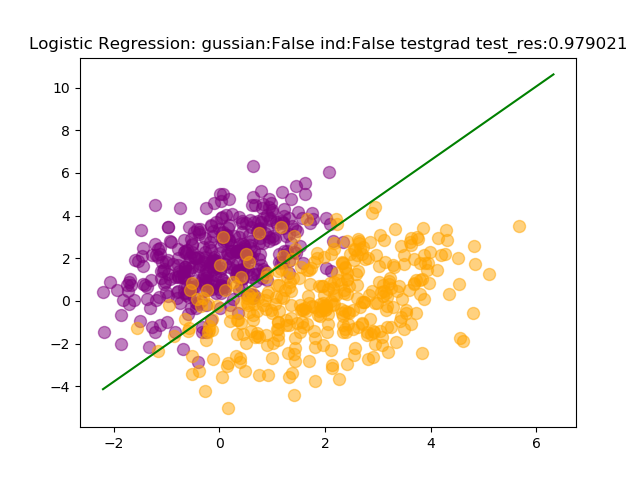
\includegraphics[width=1.2\textwidth]{pic/LogisticRegression_gussian=Falseind=Falsetestgrad.png}
    \caption{GD:no reg value not indepentent}
    \label{fig:GD no reg value not indepentent}
    \end{minipage}
    \hfill
    \begin{minipage}[t]{0.4\linewidth}
    \centering
    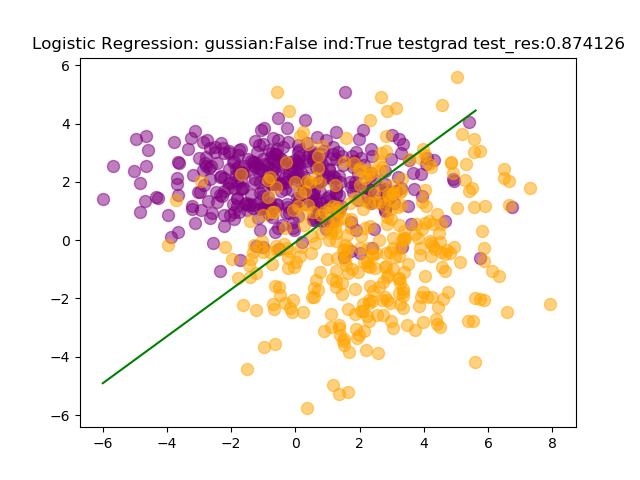
\includegraphics[width=1.2\textwidth]{pic/LogisticRegression_gussian=Falseind=Truetestgrad.png}
    \caption{GD:no reg value indepentent}
    \label{fig:GD:no reg value indepentent}
    \end{minipage}
    \\
    \begin{minipage}[t]{0.4\linewidth}
    \centering
    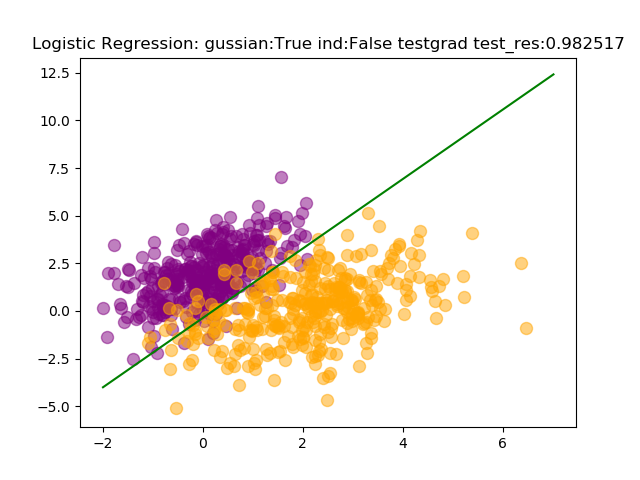
\includegraphics[width=1.2\textwidth]{pic/LogisticRegression_gussian=Trueind=Falsetestgrad.png}
    \caption{GD:with reg value not indepentent}
    \label{fig:GD:with reg value not indepentent}
    \end{minipage}
    \hfill
    \begin{minipage}[t]{0.4\linewidth}
    \centering
    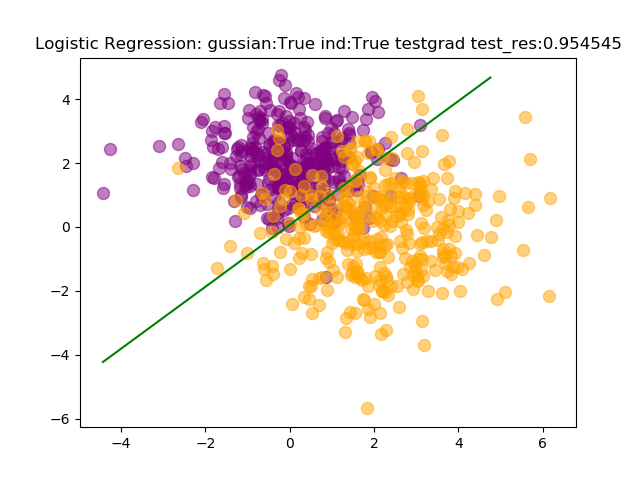
\includegraphics[width=1.2\textwidth]{pic/LogisticRegression_gussian=Trueind=Truetestgrad.png}
    \caption{GD:with reg value indepentent}
    \label{fig:GD:with reg value indepentent}
    \end{minipage}
\end{figure}



\begin{figure}[h]
    \begin{minipage}[t]{0.4\linewidth}
    \centering
    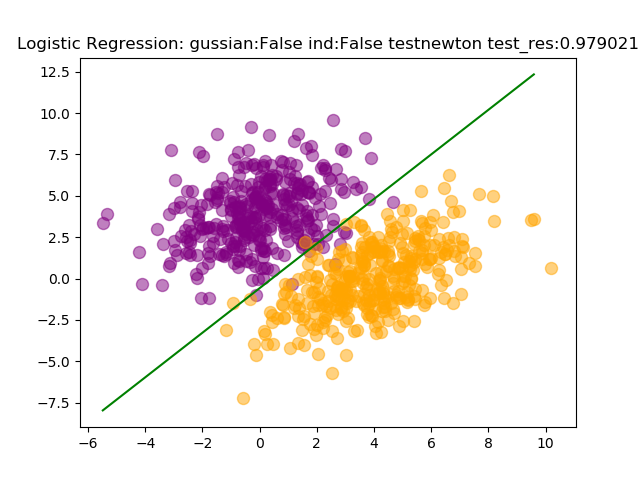
\includegraphics[width=1.2\textwidth]{pic/LogisticRegression_gussian=Falseind=Falsetestnewton.png}
    \caption{Newton: no reg val not independent}
    \label{fig:Newton: no reg val not independent}
    \end{minipage}
    \hfill
    \begin{minipage}[t]{0.4\linewidth}
    \centering
    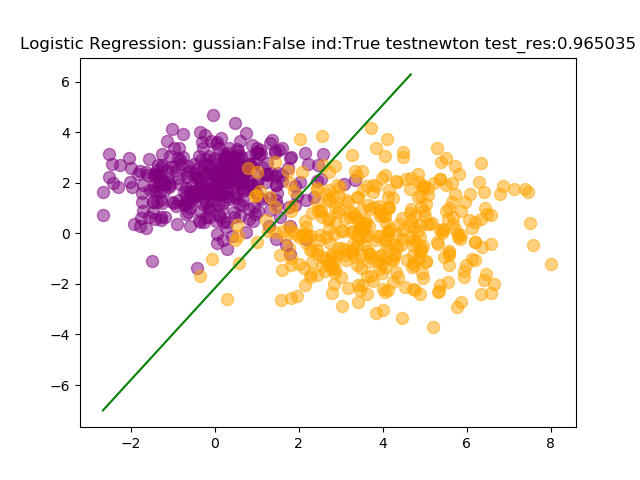
\includegraphics[width=1.2\textwidth]{pic/LogisticRegression_gussian=Falseind=Truetestnewton.png}
    \caption{Newton: no reg val independent}
    \label{fig:Newton: no reg val independent}
    \end{minipage}
\end{figure}
\begin{figure}[h]
    \begin{minipage}[t]{0.4\linewidth}
    \centering
    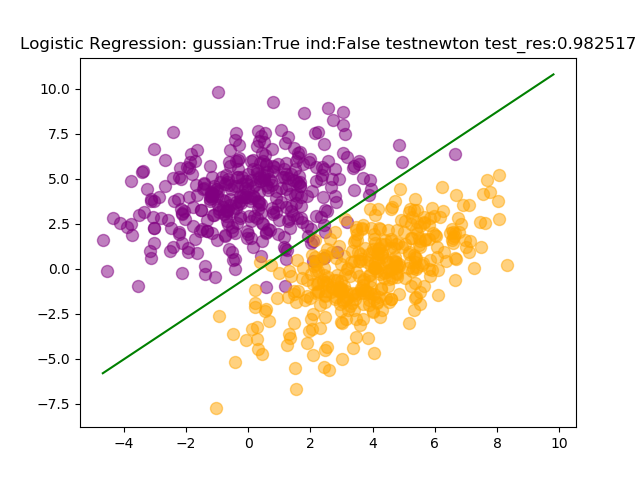
\includegraphics[width=1.2\textwidth]{pic/LogisticRegression_gussian=Trueind=Falsetestnewton.png}
    \caption{Newton: with reg val not independent}
    \label{fig:Newton: with reg val not independent}
    \end{minipage}
    \hfill
    \begin{minipage}[t]{0.4\linewidth}%9
    \centering
    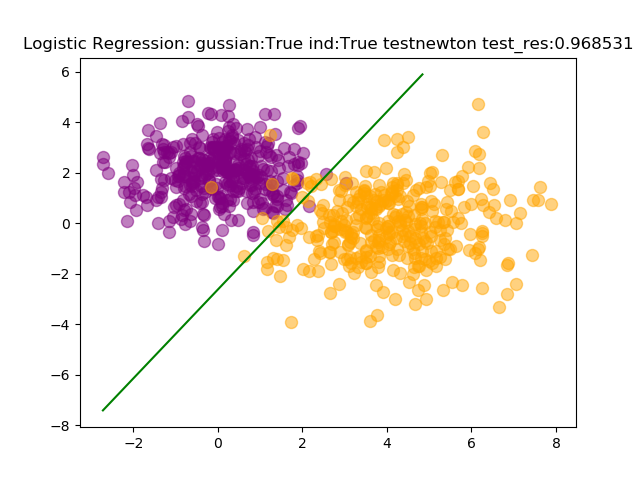
\includegraphics[width=1.2\textwidth]{pic/LogisticRegression_gussian=Trueind=Truetestnewton.png}
    \caption{Newton:with reg val independent}
    \label{fig:Newton:with reg val independent}
    \end{minipage}
\end{figure}
\subsection{Newton's method of Gradient Descent}
图5-8为Newton法用于对Loss的最小值求解,比较于直接的Gradient Descent,Newton法收敛更快。

\subsection{Test with Wine classify data from UCI}
测试数据来自UCI的\href{https://archive.ics.uci.edu/ml/machine-learning-databases/wine}{wine data}, 该数据将红酒分为三类:1,2,3,并度量相应的指标,相关指标一共13 类,因此,W矩阵维数为14,13个度量为:
\linespread{0.5}
\begin{enumerate}
\item Alcohol
\item Malic acid
\item Ash
\item Alcalinity of ash
\item Magnesium
\item Total phenols
\item Flavanoids
\item Nonflavanoid phenols
\item Proanthocyanins
\item Color intensity
\item Hue
\item OD280/OD315 of diluted wines
\item Proline
\end{enumerate}
可以将此数据划分为三类,利用逻辑递归,首先度量分类类别1,由梯度下降法得出相应的W矩阵,再计算类别2的矩阵,由这两个参数向量,可以采用决策树的结构来预测这三个分类(由于原代码实现的方式为2分类)得出结果预测准确率为0.70.

\section{结论}
\linespread{0.5}
\begin{enumerate}
\item 利用多维的高斯分布模型,通过调整COV矩阵的元素可以生成变量间相关与无关的数据分布,在描点后的状态为椭圆(有无偏斜)与正圆。
\item Newton法利用导数生成函数求最低点的方式逼近原函数的最值点,可以极大的加快模型拟合速度,但在维度过高时会出现由于Hessian阵求逆带来的浮点误差问题,导致模型发散,可以用拟牛顿法解决。
\item Logistic Regression可以对分类问题做出很好的拟合效果,正则项添加后可增强模型的泛化能力,而变量之间的条件独立性虽为Logistic Regression的推导条件之一,但对模型的拟合效果影响不大。
\end{enumerate}

\section{参考文献}
\bibliographystyle{plain} 
\bibliography{books.bib} 
\cite{ML}
\cite{PRML}

\section{Codes}





\lstset{
   aboveskip=1ex,
   backgroundcolor=\color{gray!25},
   basicstyle=\small\ttfamily,
   belowskip=1ex,
   breaklines=true,
   columns=fullflexible,
   framerule=0pt,
   framexrightmargin=0em,
   framexleftmargin=0em,
   numbers=left,
   numberstyle=\footnotesize\sffamily,
   tabsize=2
}

\begin{lstlisting}[language={Python},title={hyperparams.py}]

import numpy as np
import random
import matplotlib.pyplot as plt


class logistic(object):
    def __init__(self, xdim=2, Wgaussian_hypo=False, independent=True):
        self.gussian = Wgaussian_hypo
        self.X_vdim = xdim  # dim = 1+xdim: exp(WTX)
        self.xvalue_independent = independent
        self.X_data = None
        self.X_test = None
        self.X = None
        self.test_label = None
        self.Y = None  # X:(dim, L)=X_data.T X_data:(L, dim) Y:(L, 1) X_test:(dim, l_test)
        self.global_value_initializer()

    def global_value_initializer(self):
        """
            Automatically generate train/test matrixes, if have the input from outside, apply val directly.
        """
        if self.xvalue_independent and self.X_vdim == 2:
            pos = np.random.multivariate_normal([0, 2], cov=[[1, 0], [0, 1]], size=500)  # pos
            neg = np.random.multivariate_normal([4, 0], cov=[[2, 0], [0, 2]], size=500)  # neg
        elif not self.xvalue_independent and self.X_vdim == 2:
            pos = np.random.multivariate_normal([0, 4], [[3, 1], [1, 4]], size=500)
            neg = np.random.multivariate_normal([4, 0], [[3, 2], [2, 4]], size=500)
        else:
            pos, neg = [], []
        mapping = [([1]+list(item1), 0) for item1 in pos]
        for item in neg:
            mapping.append(([1]+list(item), 1))
        np.random.shuffle(mapping)
        self.Y = []
        self.X_data = []
        for item in mapping:  # shuffle: reduce
            self.X_data.append(item[0])
            self.Y.append(item[1])
        self.X_test = np.matrix(self.X_data[int(len(self.X_data)*5/7):]).T
        self.X_data = np.matrix(self.X_data[:int(len(self.X_data)*5/7)])
        self.X = self.X_data.T
        self.test_label = np.matrix(self.Y[int(len(self.Y)*5/7):]).T
        self.Y = np.matrix(self.Y[:int(len(self.Y)*5/7)]).T

    def generate_W(self):
        return np.matrix([random.gauss(0, 0.1) for i in range(self.X_vdim+1)]).T

    def crossMatrix(self, X): # x: (?, dim): self.X.T, matrix
        """
            Generate Matrix:(Xi*Xj) for each sample l, return val: matrix(dim, dim, L)
        """
        ans = []
        for s in range(np.size(X, 0)):
            tmpans = []  # X[s]: matrix(1, dim)
            mask = np.eye(np.size(X, 1))
            for i in range(np.size(X, 1)):
                tmpans.append([np.sum(np.dot(X[s], mask[i].T)*np.dot(X[s], mask[j].T)) for j in range(np.size(X, 1))])
            ans.append(tmpans)
        return ans

    def Loss(self, W):
        return np.array(self.Y)*np.array(np.dot(self.X.T, W)) - np.log(1 + np.exp(np.dot(W.T, self.X))).T

    def gradLoss(self, W):  # W:(dim,1) Xi:(dim, 1) Y:(L, 1), X:(dim, L )
        return np.dot(self.X, (self.Y.T - (np.exp(np.dot(W.T, self.X))/(1 + np.exp(np.dot(W.T, self.X))))).T)

    def gradgradLoss(self, W):
        val = np.exp(np.dot(W.T, self.X))
        factor = (val/(np.array(1 + val)*np.array(1 + val))).T
        cross = self.crossMatrix(self.X.T)
        hessian = np.matrix(cross[0])*np.sum(factor[0])
        for i in range(1, np.size(factor, 0)):
            hessian += np.matrix(cross[i])*np.sum(factor[i])
        return hessian

    def newton_log(self, threshold=1e-8, alpha=1, lambdas=1e-2):
        W, val_hold = self.generate_W(), 0  # (dim, 1)
        while True:
            step = np.dot(self.gradgradLoss(W).I, self.gradLoss(W))
            if self.gussian:
                W += alpha*(step - lambdas*W)
            else:
                W += alpha*step
            print(W, np.sum(self.gradLoss(W)))
            if abs(np.sum(self.gradLoss(W))) <= threshold or val_hold - np.sum(self.gradLoss(W)) < 1e-5:
                break
            else: val_hold = np.sum(self.gradLoss(W))
        print(self.gradLoss(W))
        return W

    def gradient_descent(self, threshold=1e-4, alpha=5e-8, lambdas=1e-2):
        W = self.generate_W()
        while True:
            step = self.gradLoss(W)
            if self.gussian:
                W += alpha*(step - lambdas*W)
            else:
                W += alpha*step
            print(W)
            print(np.sum(self.gradLoss(W)))
            if abs(np.sum(self.gradLoss(W))) <= threshold:
                break
        return W

    def test(self, W):
        val = (1/(1+np.exp(np.dot(W.T, self.X_test)))).T
        expect = [int(np.sum(val[i]) < 0.5) for i in range(np.size(val, 0))]
        return 1 - abs(np.sum(abs(expect - self.test_label.T))/np.size(val, 0))

    def pr_plot(self, W, flag=""):
        if self.X_vdim == 2:
            w0, w1, w2 = np.sum(W[0]), np.sum(W[1]), np.sum(W[2])
            plt_X = np.linspace(np.min(self.X[1]), np.max(np.max(self.X[2])))
            plt_Y = [-w0/w2 - w1/w2*x for x in plt_X]
            mask = np.eye(3)
            scatter = [(np.sum(np.dot(item, mask[1])), np.sum(np.dot(item, mask[2]))) for item in self.X_data]
            print(scatter)
            label_pt = self.Y.T
            scat_pos = [[], []]
            scat_neg = [[], []]
            for i in range(len(scatter)):
                if np.sum(self.Y[i]) == 0:
                    scat_neg[0].append(scatter[i][0])
                    scat_neg[1].append(scatter[i][1])
                elif np.sum(self.Y[i]) == 1:
                    scat_pos[0].append(scatter[i][0])
                    scat_pos[1].append(scatter[i][1])
                else:
                    print("Error while map/reduce the points.")
            plt.scatter(scat_neg[0], scat_neg[1], s=75, alpha=.5, color='purple')
            plt.scatter(scat_pos[0], scat_pos[1], s=75, alpha=.5, color='orange')
            plt.plot(plt_X, plt_Y, color='green')
            plt.title("Logistic Regression: gussian:%s ind:%s %s test_res:%f" % (str(self.gussian), str(self.xvalue_independent), flag, self.test(W)))
            plt.savefig("LogisticRegression_gussian=%sind=%s%s.png" % (str(self.gussian), str(self.xvalue_independent), flag))
            plt.show()
        else:
            pass  # go to test


def wine_data_insert():
    f = open("winedata.csv", "r")
    classify, classify_test, X_data, X_test = [], [], [], []
    for line in f:
        line = line.split(",")
        # if int(line[0]) == 3: continue
        classify.append(int(line[0]) - 1)
        tmp = [1]
        for i in range(1, len(line)):
            tmp.append(float(line[i]))
        X_data.append((tmp, int(line[0]) - 1))
    random.shuffle(X_data)
    X_test = X_data[int(len(X_data)*5/7):]
    classify_test = [item[1] for item in X_test]
    X_test = [item[0] for item in X_test]
    X_data = X_data[:int(len(X_data)*5/7)]
    classify = [item[1] for item in X_data]
    X_data = [item[0] for item in X_data]
    f, fl = open("wine_test.txt", "w"), open("wine_test_label.txt", "w")
    for (item, label) in zip(X_test, classify_test):
        for it in item: f.write(str(it) + "\t")
        f.write("\n")
        fl.write(str(label) + "\n")
    f.close(), fl.close()
    fr, frl = open("wine_train.txt", "w"), open("wine_train_label.txt", "w")
    for (item, label) in zip(X_data, classify):
        for it in item: fr.write(str(it) + "\t")
        fr.write("\n")
        frl.write(str(label) + "\n")
    fr.close(), frl.close()
    return np.matrix(X_data), np.matrix(X_test).T, np.matrix(classify).T, np.matrix(classify_test).T


def ReadFromStandardFile(mask=0):
    X_train, X_test, Y_train, Y_test = [], [], [], []
    f, fl = open("wine_test.txt", "r"), open("wine_test_label.txt", "r")
    for line in f:
        line = line.split()
        X_test.append([float(line[i]) for i in range(0, len(line))])
    for line in fl:
        if mask != -1: Y_test.append([int(float(line) == mask)])
        else: Y_test.append([int(line)])
    fr, frl = open("wine_train.txt", "r"), open("wine_train_label.txt", "r")
    for line in fr:
        print(line)
        line = line.split()
        X_train.append([float(line[i]) for i in range(0, len(line))])
    for line in frl:
        Y_train.append([int(float(line) == mask)])
    return np.matrix(X_train), np.matrix(Y_train), np.matrix(X_test).T, np.matrix(Y_test)


def decision_tree():  # precision: 0.705882
    # classify label 1 first(original:2), then classify label 0 (ori:1), the other point is label 2 (ori:3)
    W_cl1 = [[-0.19624184], [0.14048495], [-0.32750738], [0.04732983], [0.1123163], [0.02439485], [0.0467235],
             [0.09784779], [0.04087847], [-0.18535481], [-0.23524893], [-0.08212339], [-0.05971632], [-0.00696094]]
    W_cl0 = [[0.0187151], [0.00048866], [-0.10105207], [0.06552508], [-0.46800525], [-0.04441048], [-0.02615863],
             [0.13665488], [0.08469632], [-0.00764128], [-0.05588578], [-0.02218694], [0.03718035], [0.01629198]]
    W_cl1 = np.matrix(W_cl1)
    W_cl0 = np.matrix(W_cl0)
    X_test, Y_test = [], []
    f, fl = open("wine_test.txt", "r"), open("wine_test_label.txt", "r")
    for line in f:
        line = line.split()
        X_test.append([float(line[i]) for i in range(0, len(line))])
    for line in fl:
        Y_test.append(int(line))
    X_test = np.matrix(X_test).T
    val1 = (1/(1+np.exp(np.dot(W_cl1.T, X_test)))).T
    expect1 = [int(np.sum(val1[i]) < 0.5) for i in range(np.size(val1, 0))]
    val0 = (1/(1+np.exp(np.dot(W_cl0.T, X_test)))).T
    expect0 = [int(np.sum(val0[i]) < 0.5) for i in range(np.size(val0, 0))]
    print(expect0)
    print(expect1)
    print(Y_test)
    ans = []
    for i in range(0, len(expect0)):
        if expect1[i] == 1:
            ans.append(1)
        elif expect0[i] == 1:
            ans.append(0)
        else:
            ans.append(2)
    cnt = 0
    print(ans)
    for i in range(0, len(ans)):
        if ans[i] == Y_test[i]:
            cnt += 1
    print("Precision = %lf" % (cnt/len(ans)))
    return cnt/len(ans)


if __name__ == "__main__":
    """
        Normal Train, test
    """
    log = logistic(Wgaussian_hypo=True, independent=True)
    w = log.gradient_descent()
    print("RES:")
    print(w)
    log.pr_plot(w, "testgrad")

    """
        Train, test from dataset: UCI: https://archive.ics.uci.edu/ml/machine-learning-databases/wine
        classify 0: W :0.90196
        [[ 0.11116817]
        [-0.18515697]
        [ 0.05445636]
        [-0.07500515]
        [-0.41380713]
        [-0.03442779]
        [ 0.09983258]
        [ 0.01055378]
        [-0.01554494]
        [ 0.02209726]
        [-0.07036363]
        [ 0.0266265 ]
        [ 0.0548774 ]
        [ 0.01650266]]
        classify:1 W :0.882352941176
        [[ 0.0088141 ]
        [ 0.00994699]
        [-0.1510287 ]
        [ 0.0400127 ]
        [ 0.15663027]
        [ 0.02726139]
        [ 0.10969113]
        [ 0.27900054]
        [ 0.06219452]
        [ 0.15556723]
        [-0.54909899]
        [ 0.12975475]
        [ 0.2285545 ]
        [-0.0077714 ]]
    class 2: 0.90196
    
    class 1-> 0: 0.705882

    Wine data/classification below:
    """
    log = logistic(xdim=13)
    # log.X_data, log.X_test, log.Y, log.test_label = wine_data_insert()
    log.X_data, log.Y, log.X_test, log.test_label = ReadFromStandardFile(mask=2)  # 1
    log.X = log.X_data.T
    print(log.X)
    print(log.Y)
    print(log.test_label)
    w = log.gradient_descent(threshold=1e-5)
    print(log.test(w))
    decision_tree()

\end{lstlisting}


\section{End}
Machine Learning: Logistic Regression\\

Copyright \textcopyright RuiKang(\href{https://github.com/marisuki}{marisuki}) 2018

\end{document}

